\documentclass[a4paper,10pt]{article}

% ---- Encoding ---------------------------------------------------------------
\usepackage[utf8]{inputenc}

% --- Langage -----------------------------------------------------------------
\usepackage[american]{babel}


% --- Various packages --------------------------------------------------------
\usepackage{ifthen}
\usepackage{marginnote}
\usepackage{tikz}
\usepackage{framed}
\usepackage{lipsum}


% --- Mathematics -------------------------------------------------------------
\usepackage{amsmath}

% --- Page layout -------------------------------------------------------------
\usepackage[a4paper]{geometry}
\geometry{left=1.5cm, right=1.5cm, height=28cm}
\geometry{footskip=1.25cm, headheight=1cm, headsep=1.25cm}
\geometry{marginparsep=0.5cm, marginpar=5cm}
\geometry{includehead, includefoot, includemp}


% --- Font stack --------------------------------------------------------------
\usepackage{mathpazo}   % Roman & math
\usepackage[scale=0.95]{FiraSans}   % Sans Serif
\usepackage[varqu]{zi4} % Monotype


% --- Colors ------------------------------------------------------------------
\usepackage{xcolor}
\definecolor{darkred}{HTML}{CF232B}
\definecolor{darkblue}{HTML}{2B23CF}
\definecolor{darkgray}{HTML}{555555}
\definecolor{lightgray}{HTML}{F9F9F9}

%\definecolor{citecolor}{HTML}{EB811B}
\colorlet{citecolor}{darkblue}
\colorlet{linkcolor}{citecolor}
\colorlet{urlcolor}{citecolor}


% -- Section titles & ToC -----------------------------------------------------
\usepackage{sectsty}
\allsectionsfont{\sffamily\bfseries}

\usepackage{tocloft}
\renewcommand{\thesection}{}
\renewcommand{\cftsecfont}{\sffamily}
\renewcommand{\cftsecleader}{\cftdotfill{\cftdotsep}}

\setcounter{tocdepth}{1}

% With babel
\addto\captionsamerican{
  \renewcommand{\contentsname}
    {\normalsize \sf \bfseries Contents}%
}
% Without babel
% \renewcommand{\contentsname}{}

\makeatletter
\def\@seccntformat#1{\csname #1ignore\expandafter\endcsname\csname the#1\endcsname\quad}
\let\sectionignore\@gobbletwo
\let\latex@numberline\numberline
\def\numberline#1{\if\relax#1\relax\else\latex@numberline{#1}\fi}
\makeatother

% --- Sidenotes ---------------------------------------------------------------
\usepackage{sidenotes}
% Used in \sidenote
% Changed to meet the question of user J. Bratt
%  (https://tex.stackexchange.com/questions/361622).
\makeatletter
\RenewDocumentCommand \sidenotetext { o o +m }
{\IfNoValueOrEmptyTF{#1}{
\@sidenotes@placemarginal{#2}{\textsuperscript{\sf\thesidenote}{}~\sf\footnotesize#3}
\refstepcounter{sidenote}}
{\@sidenotes@placemarginal{#2}{\textsuperscript{#1}~#3}}}
\makeatother


% --- Captions ----------------------------------------------------------------
\usepackage[labelsep=period]{caption}
\renewcommand{\captionfont}{\small}
\renewcommand{\captionlabelfont}{\small\sffamily\bfseries}
\captionsetup[figure]{justification=justified, singlelinecheck=false}


% --- Hyperref & colors -------------------------------------------------------
\usepackage[pdfusetitle,
            bookmarks=true,
            breaklinks=true,
            pdfborder={0 0 0},
            citecolor=citecolor,
            linkcolor=linkcolor,
            urlcolor=urlcolor,
            colorlinks=true,
            linktocpage=false,
            hyperindex=true,
            colorlinks=true,
            linktocpage=false,
            linkbordercolor=white]{hyperref}
\urlstyle{sf}


% --- Listings ----------------------------------------------------------------
\usepackage{listings}
\lstset{%
  % language={Latex},
  basicstyle=\ttfamily\small,
  keywordstyle=\color{mLightBrown}\bfseries,
  commentstyle=\color{mLightGreen},
  stringstyle=\color{mLightGreen},
  backgroundcolor=\color{lightgray},
  numbers=none,
  numberstyle=\ttfamily,
  stepnumber=2,
  showspaces=false,
  showstringspaces=false,
  showtabs=false,
  frame=none,
  framerule=0.5pt,
  tabsize=2,
  rulesep=5em,
  captionpos=b,
  breaklines=true,
  breakatwhitespace=false,
  framexleftmargin=0.em,
  xleftmargin=0.0em,
  framexrightmargin=0.0em,
  xrightmargin=0em,
  aboveskip=0.5em,
  belowskip=0.5em,
}

% --- Bibliography ------------------------------------------------------------
\usepackage[
  backend=biber,
  style = numeric,
  % style=authoryear,
  sorting = none,
  giveninits = true,
  maxcitenames=3,
  mincitenames=1,
  maxbibnames=10,
  isbn = false,
  url = false,
  doi = false,
  autocite = superscript,
  natbib = true]{biblatex}
\usepackage{bibentry}
\DeclareFieldFormat{labelnumberwidth}{#1\adddot}

% Side margin cite 
\newcommand{\sidecite}[1]{\marginpar{\sf\scriptsize\fullcite{#1}}}


% --- Layout ------------------------------------------------------------------
% No indentation at beginning of a new paragraph
\setlength\parindent{0pt}

% No space between items in itemize and enuemrate lists
\usepackage{enumitem}
\setlist[itemize]{noitemsep}
\setlist[enumerate]{noitemsep}


% --- Authors block -----------------------------------------------------------
\usepackage{authblk,etoolbox}

\makeatletter
% patch \maketitle so that it doesn't center
\patchcmd{\@maketitle}{center}{flushleft}{}{}
\patchcmd{\@maketitle}{center}{flushleft}{}{}
% patch \maketitle so that the font size for the title is normal
\patchcmd{\@maketitle}{\LARGE}{\Large\sf\bfseries\vspace{-2.5em}}{}{}

% patch the patch by authblk so that the author block is flush left
\def\maketitle{{%
  \renewenvironment{tabular}[2][]
    {\begin{flushleft}}
    {\end{flushleft}}
  \AB@maketitle}}
\makeatother

\setlength{\affilsep}{0.25em}
\renewcommand\Affilfont{\normalfont\sf\footnotesize}
\renewcommand\Authfont{\sf\bfseries\small}
\renewcommand\Authands{\normalfont\sf\small}


% --- Various convenient macros -----------------------------------------------
\usepackage[many]{tcolorbox}
\newtcbox{\iconbox}[1][]{%
  enhanced,nobeforeafter,tcbox raise base, 
  boxrule=0.4pt, top=0pt, bottom=-1pt,
  right=1pt, left=1pt, arc=1pt, boxsep=1pt,
  fontupper={\tiny \sffamily}, before upper={\vphantom{dlg}},
  colframe=white, colback=black!10!white, coltext=black}
\newcommand{\orcid}[1]{\href{https://orcid.org/#1}{\iconbox{ID}}}
\newcommand{\doi}[1]{\href{http://doi.org/#1}{#1}}
\newcommand{\github}[1]{\href{https://github.com/#1}{github.com/#1}}





% --- Headers & footers -------------------------------------------------------
% DO NOT EDIT - automatically generated from metadata.yaml

\def \codeURL{https://github.com/ReScience/ReScience-template}
\def \codeDOI{10.5281/zenodo.27944}
\def \dataURL{}
\def \dataDOI{}
\def \editorNAME{Tiziano Zito}
\def \editorORCID{}
\def \reviewerINAME{Benoît Girard}
\def \reviewerIORCID{0000-0002-8117-7064}
\def \reviewerIINAME{Mehdi Khamassi}
\def \reviewerIIORCID{0000-0002-2515-1046}
\def \dateRECEIVED{09 June 2015}
\def \dateACCEPTED{12 August 2015}
\def \datePUBLISHED{14 August 2015}
\def \articleTITLE{ReScience Article Template}
\def \articleYEAR{2015}
\def \reviewURL{None}
\def \articleABSTRACT{This article is a proposition for a new article template for the ReScience C (computational replication) and ReScience X (experimental replication) journals. It is loosely based after Edward Tufte’s book style where the large left columns containes the main text and the right columns is used for auxiliary informations such as notes, captions or references. The template requires a standard TeXLive installation in order to compile it and this PDF has been compiled using TeXLive 2017 (pdflatex). Both the style, the layout and the colors of the template aim at giving ReScience a strong but subtle identity.}
\def \replicationBIB{M. Guthrie, A. Leblois, A. Garenne, and T. Boraud. Interaction between cognitive and motor cortico-basal ganglia loops during decision making: a computational study. In: Journal of Neurophysiology 109.12 (2013)}
\def \replicationDOI{10.1152/jn.00026.2013}
\def \contactNAME{Nicolas P. Rougier}
\def \contactEMAIL{Nicolas.Rougier@inria.fr}
\def \articleKEYWORDS{Latex, Template, ReScience}
\def \journalVOLUME{1}
\def \journalISSUE{1}
\def \articleNUMBER{1}
\def \articleDOI{}
\def \authorsFULL{Nicolas P. Rougier and Nicolas P. Rougier}
\def \authorsABBRV{N.P. Rougier and N.P. Rougier}
\def \authorsSHORT{Rougier and Rougier}
\title{\articleTITLE}
\date{}
\author[1,2,3,\orcid{0000-0002-6972-589X}]{Nicolas P. Rougier}
\affil[1]{INRIA Bordeaux Sud-Ouest, Bordeaux, France}
\affil[2]{LaBRI, Université de Bordeaux, Institut Polytechnique de Bordeaux, Centre National de la Recherche Scientifique, UMR 5800, Talence, France}
\affil[3]{Institut des Maladies Neurodégénératives, Université  de Bordeaux, Centre National de la Recherche Scientifique, UMR 5293, Bordeaux, France}


\newcommand{\ReScience}{\sf Re{\bfseries \textcolor{darkred}{Science C}} }

\usepackage{fancyhdr}
\usepackage{ccicons}

\pagestyle{fancy}
\fancypagestyle{plain}{}
\addtolength{\headwidth}{\marginparsep}
\addtolength{\headwidth}{\marginparwidth}
\renewcommand{\headrulewidth}{0.0pt}
\lhead{\sf \ReScience -- Rougier 2018}
\chead{\sf }
\rhead{\ifthenelse{\value{page}=1}{%
\begin{tikzpicture}[remember picture, overlay]
  \node [shift={(-3.5cm,-4cm)}] at (current page.north east) {
     \begin{tikzpicture}[remember picture, overlay]
       \fill [fill=darkred, opacity=1.0] (0,0) rectangle (2.cm,4cm);
       \node [shift={(1cm,1cm)}, opacity=1.0]
             {
\includegraphics[width=1.5cm]{logo.pdf}};
     \end{tikzpicture}
  };
\end{tikzpicture}}{\sf \large \textcolor{gray}{Editorial}}}
\renewcommand{\footrulewidth}{0.0pt}
\lfoot{\sf \today}
\cfoot{\sf }
\rfoot{
  \ifthenelse{\value{page}=1}
  {\sf \thepage}
  {\begin{tikzpicture}[remember picture, overlay]
      \node [shift={(-2.25cm,0cm)}] at (current page.south east) {
        \begin{tikzpicture}[remember picture, overlay]
          \fill [fill=darkred, opacity=1.0] (0,0) rectangle (0.75cm,1.50cm);
          \node [shift={(.375cm,1.1cm)}, color=white] {\sf \bfseries \thepage};
        \end{tikzpicture}
      };
    \end{tikzpicture}}
}


% =============================================================================
\bibliography{article.bib}

%\begin{document}
%% --- Domain ------------------------------------------------------------------
%
~\\ {\sf \large \textcolor{gray}{Editorial}}
%
% --- Title -------------------------------------------------------------------
%
{\let\newpage\relax\maketitle} \maketitle

% --- Abstract ----------------------------------------------------------------
{\sf \bfseries Abstract} \articleABSTRACT\\

% --- Keywords ----------------------------------------------------------------
{\sf \bfseries Keywords:} \articleKEYWORDS\\

% --- Replication -------------------------------------------------------------
%
\ifdefempty{\replicationBIB}{}{
{\sf \bfseries A replication of}
\ifdefempty{\replicationURL}{\href{http://doi.org/\replicationDOI}{\sf \replicationBIB}}
                            {\href{\replicationURL}{\sf \replicationBIB}}.\\}

% --- Code repository ---------------------------------------------------------
{\sf \bfseries Code:}
   \href{\codeURL}{\sf \codeURL}
   \ifdefempty{\codeDOI}{}{ -- \textbf{DOI} \doi{\codeDOI}}\\
\ifdefempty{\dataURL}{}{
  \textbf{Data:} \href{\dataURL}{\sf \dataURL}
  \ifdefempty{\dataDOI}{}{ -- \textbf{DOI} \doi{\dataDOI}}\\
}


% --- Spacing -----------------------------------------------------------------
\vfill

% --- Editor block ------------------------------------------------------------
\begin{minipage}{\headwidth}
\vfill
%\noindent\makebox[\textwidth]{\rule{\textwidth}{0.5pt}}
\begin{framed}
  \footnotesize \sf

  %% Submission only
  \ifdefempty{\articleDOI}{
%    \begin{tcolorbox}[
%        arc=0pt, boxsep=0pt, boxrule=0.5pt,
%        colframe=white,colback=darkred, coltext=white]
    \textcolor{darkred}{\large \bfseries Non peer-reviewed author version}
  }
  %% Published
  {\textbf{Cite as} \articleTITLE, \authorsABBRV.
                     In: {\em \journalNAME}
                     \journalVOLUME(\#\articleNUMBER), \articleYEAR.
                     \ifdefempty{\articleDOI}{}{\textbf{DOI} \doi{\articleDOI}}.\par}

% --- Code --------------------------------------------------------------------
%% \textbf{Code repository} at \href{\codeURL}{\codeURL}
%%                             \ifdefempty{\codeDOI}{}{ -- \textbf{DOI} \doi{\codeDOI}}\\
% --- Data --------------------------------------------------------------------
%% \ifdefempty{\dataURL}{}{
%%   \textbf{Data repository} at \href{\dataURL}{\dataURL}
%%   \ifdefempty{\dataDOI}{}{ -- \textbf{DOI} \doi{\dataDOI}}\\
%% }
%%~\\
% --- Editor --------------------------------------------------------------------
\ifdefempty{\editorNAME}{}{
  \textbf{Edited by}
  \editorNAME\ifdefempty{\editorORCID}{}{$^{\orcid{\editorORCID}}$} --
  \textbf{Reviewed by}
  \reviewerINAME\ifdefempty{\reviewerIORCID}{}{$^{\orcid{\reviewerIORCID}}$}
  \&
  \reviewerINAME\ifdefempty{\reviewerIIORCID}{}{$^{\orcid{\reviewerIIORCID}}$}
  \href{\reviewURL}{\sf \bfseries Open Review}\par
}
%
% --- Dates --------------------------------------------------------------------
\ifdefempty{\dateRECEIVED}{}{
  \textbf{Received}  \dateRECEIVED
  \ifdefempty{\dateACCEPTED}{}{-- \textbf{Accepted}\dateACCEPTED}
  \ifdefempty{\datePUBLISHED}{}{-- \textbf{Accepted}\datePUBLISHED}\\}

% --- Copyright --------------------------------------------------------------------
\textbf{Copyright} ©~\articleYEAR~\authorsABBRV\par
\textbf{Published} under a Creative Commons Attribution 4.0 International license
\href{https://creativecommons.org/licenses/by/4.0/}{\ExternalLink}\par
%
\textbf{Corresponding author}:
\contactNAME~(\href{mailto:\contactEMAIL}{\contactEMAIL})\\
\textbf{Competing Interests}:
The authors have declared that no competing interests exist\par
\end{framed}
%}

  
%\begin{tikzpicture}[remember picture, overlay]
  \node [shift={(+1.5cm,-4cm)}] at (current page.north west) {
     \begin{tikzpicture}[remember picture, overlay]
       \fill [fill=red, opacity=1.0] (0,0) rectangle (2.cm,4cm);
       \node [shift={(1cm,1cm)}, opacity=1.0]
             {
\includegraphics[width=1.5cm]{logo.pdf}};
     \end{tikzpicture}
  };
\end{tikzpicture}

%% \begin{tikzpicture}[remember picture, overlay]
%%   \node [shift={(+0cm,-2.5cm)}] at (current page.north west) {
%%      \begin{tikzpicture}[remember picture, overlay]
%%        \fill [fill=red, opacity=1.0] (0,0) rectangle (2.5cm,2.5cm);
%%        \node [shift={(1.25cm,1.5cm)}, opacity=1.0]
%%              {
\includegraphics[width=1.5cm]{logo.pdf}};
%%        \node [color=white, shift={(1.25cm,.4cm)}]
%%              {\footnotesize \sffamily \scshape \bfseries ReScience C};
%%      \end{tikzpicture}
%%   };
%% \end{tikzpicture}


\vfill
\noindent\makebox[\textwidth]{\rule{\textwidth}{0.4pt}}
{\footnotesize \sf
  \noindent \textbf{Cite as}: \articleTITLE, \authorsABBRV.
                              In: {\em ReScience C}
                              \journalVOLUME(\#\articleNUMBER), \articleYEAR.
                              \textbf{DOI} \doi{\articleDOI}.\par
~\\
\noindent \textbf{Code repository} at \href{https://\codeURL}{\codeURL} --
          \textbf{DOI}                \doi{\codeDOI}\\
\ifdefempty{\dataURL}{}{
\noindent \textbf{Data repository} at \href{https://\dataURL}{\dataURL} --
          \textbf{DOI}                \doi{\dataDOI}\\
}
~\\
\noindent \textbf{Edited by}   \editorNAME$^{\orcid{\editorORCID}}$ --
          \textbf{Reviewed by} \reviewerINAME$^{\orcid{\reviewerIORCID}}$ 
           \&                  \reviewerIINAME$^{\orcid{\reviewerIIORCID}}$ --
                               \href{\reviewURL}{Open Review}\par
\noindent \textbf{Received}  \dateRECEIVED~--
          \textbf{Accepted}  \dateACCEPTED~--
          \textbf{Published} \datePUBLISHED\par
\noindent \textbf{Copyright} ©~\articleYEAR~\authorsABBRV\par
\noindent \textbf{Published} under a Creative Commons Attribution 4.0 International
          (\href{https://creativecommons.org/licenses/by/4.0/}{\ccLogo\ccAttribution})
          license\par
~\\
\noindent \textbf{Corresponding author}:
\contactNAME~(\href{mailto:\contactEMAIL}{\contactEMAIL})\\
\noindent \textbf{Competing Interests}:
           The authors have declared that no competing interests exist\par
}
\clearpage

%\sf \footnotesize \lipsum[1-2]
\end{minipage}


\clearpage


%\section*{Introduction}

What a nice template\footnote{I did it myself!} for \citep{Rougier:2017}
\marginpar{\sf \footnotesize Margin note can be used to insert a message in the
  margin such as for example a reference: \fullcite{Rougier:2017}}. \lipsum*[1]


\subsection*{Figures}

\begin{figure}[htbp]
   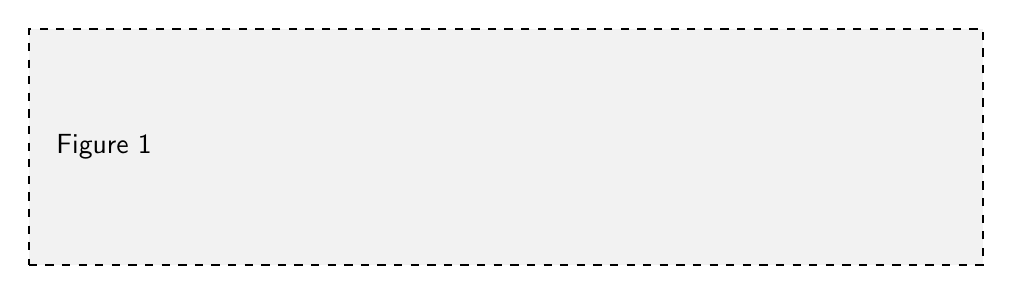
\begin{tikzpicture}
     \node[draw, fill=black!5, dashed, thick,
       text width=.98\textwidth, minimum height=3cm] at (0,0) {~~\sf Figure 1};
   \end{tikzpicture}
    \captionof{figure}{Figure caption.}
    \label{fig:1}
\end{figure}

\subsection*{Tables}
\begin{table}[htbp]
\begin{minipage}{.45\textwidth}
  \begin{tabularx}{\textwidth}{|XX|}
      \hline
      \bfseries Header 1 & \bfseries Header 2\\
      \hline
      Item 1 & Item 2\\
      Item 1 & Item 2\\
      Item 1 & Item 2\\
      \hline
    \end{tabularx}
    \captionof{table}{Table caption.}
    \label{tab:1}
\end{minipage}
\hfill
\begin{minipage}{.45\textwidth}
  \begin{tabularx}{\textwidth}{|XX|}
      \hline
      \bfseries Header 1 & \bfseries Header 2\\
      \hline
      Item 1 & Item 2\\
      Item 1 & Item 2\\
      Item 1 & Item 2\\
      \hline
    \end{tabularx}
    \captionof{table}{Table caption.}
    \label{tab:2}
\end{minipage}
\end{table}

\subsection*{Equations}
The well known Pythagorean theorem \(x^2 + y^2 = z^2\) was proved to be invalid
for other exponents.  Meaning equation \eqref{eq:1} has no integer solutions:
%%
\begin{equation}
  \label{eq:1}
  x^n + y^n = z^n
\end{equation}
\marginpar{\sf \footnotesize
           \vspace{-4em} I have a proof but it doesn't fit in the margin...}


\subsection*{Listings}
\begin{lstlisting}[language=python,
                   caption={Listing caption.},
                   label={lst:1}]
# Standard import
import this

text = "Some text"
\end{lstlisting}


\section*{Conclusion}

This is a short article.\\

\lipsum*[2]\\

%\addcontentsline{toc}{section}{References}
%\renewcommand*{\bibfont}{\footnotesize \sffamily}
%\printbibliography
%\end{document}
% =============================================================================


\begin{document}
\vspace{.5em}
{\sf \large \textcolor{gray}{Editorial}}
\marginpar{
\vspace{4em}
\begin{tcolorbox}[% width=\textwidth, % height=3cm,
                  arc=1pt, boxsep=0pt, boxrule=1pt,
                  colframe=darkred!25!white,
                  colback=darkred!10!white,
                  coltext=black]
  {\sf \small
      {\bfseries Author version}\\
      {\footnotesize Submitted on \today}}
\end{tcolorbox}
}

{\let\newpage\relax\maketitle}
\maketitle

{\sf \bfseries Abstract} This article is a proposition for a new
article template for the ReScience C (computational replication) and ReScience
X (experimental replication) journals. It is loosely based after Edward Tufte's
book style where the large left columns containes the main text and the right
columns is used for auxiliary informations such as notes, captions or
references. The template requires a standard TeXLive installation in order to
compile it and this PDF has been compiled using TeXLive 2017 (pdflatex). Both
the style, the layout and the colors of the template aim at giving ReScience a
strong but subtle identity.\\

{\sf \bfseries Keywords} Latex, Template, ReScience\\

\renewcommand{\baselinestretch}{0.5}\normalsize
\tableofcontents
\renewcommand{\baselinestretch}{1.0}\normalsize

%% \vspace{5mm}
%% {\small \sf {\bfseries Contact}: 
%% Nicolas P. Rougier (\href{mailto:nicolas.rougier@inria.fr}{nicolas.rougier@inria.fr})}

\vfill


\begin{minipage}{\headwidth}
\vfill
\noindent\makebox[\textwidth]{\rule{\textwidth}{0.5pt}}
{\footnotesize \sf
  \noindent \textbf{Cite as} \articleTITLE, \authorsABBRV.
                             In: {\em ReScience C}
                             \journalVOLUME(\#\articleNUMBER), \articleYEAR.
                             \textbf{DOI} \doi{\articleDOI}.\par
~\\
\noindent \textbf{Code repository} at \href{https://\codeURL}{\codeURL} --
          \textbf{DOI}                \doi{\codeDOI}\\
\ifdefempty{\dataURL}{}{
\noindent \textbf{Data repository} at \href{https://\dataURL}{\dataURL} --
          \textbf{DOI}                \doi{\dataDOI}\\
}
~\\
\noindent \textbf{Edited by}   \editorNAME$^{\orcid{\editorORCID}}$ --
          \textbf{Reviewed by} \reviewerINAME$^{\orcid{\reviewerIORCID}}$ 
           \&                  \reviewerIINAME$^{\orcid{\reviewerIIORCID}}$ --
                               \href{\reviewURL}{Open Review}\par
\noindent \textbf{Received}  \dateRECEIVED~--
          \textbf{Accepted}  \dateACCEPTED~--
          \textbf{Published} \datePUBLISHED\par
\noindent \textbf{Copyright} ©~\articleYEAR~\authorsABBRV\par
\noindent \textbf{Published} under a Creative Commons Attribution 4.0 International
          (\href{https://creativecommons.org/licenses/by/4.0/}{\ccLogo\ccAttribution})
          license\par
~\\
\noindent \textbf{Corresponding author}:
\contactNAME~(\href{mailto:\contactEMAIL}{\contactEMAIL})\\
\noindent \textbf{Competing Interests}:
           The authors have declared that no competing interests exist\par
}

  
%\begin{tikzpicture}[remember picture, overlay]
  \node [shift={(+1.5cm,-4cm)}] at (current page.north west) {
     \begin{tikzpicture}[remember picture, overlay]
       \fill [fill=red, opacity=1.0] (0,0) rectangle (2.cm,4cm);
       \node [shift={(1cm,1cm)}, opacity=1.0]
             {
\includegraphics[width=1.5cm]{logo.pdf}};
     \end{tikzpicture}
  };
\end{tikzpicture}

%% \begin{tikzpicture}[remember picture, overlay]
%%   \node [shift={(+0cm,-2.5cm)}] at (current page.north west) {
%%      \begin{tikzpicture}[remember picture, overlay]
%%        \fill [fill=red, opacity=1.0] (0,0) rectangle (2.5cm,2.5cm);
%%        \node [shift={(1.25cm,1.5cm)}, opacity=1.0]
%%              {
\includegraphics[width=1.5cm]{logo.pdf}};
%%        \node [color=white, shift={(1.25cm,.4cm)}]
%%              {\footnotesize \sffamily \scshape \bfseries ReScience C};
%%      \end{tikzpicture}
%%   };
%% \end{tikzpicture}


\vfill
\noindent\makebox[\textwidth]{\rule{\textwidth}{0.4pt}}
{\footnotesize \sf
  \noindent \textbf{Cite as}: \articleTITLE, \authorsABBRV.
                              In: {\em ReScience C}
                              \journalVOLUME(\#\articleNUMBER), \articleYEAR.
                              \textbf{DOI} \doi{\articleDOI}.\par
~\\
\noindent \textbf{Code repository} at \href{https://\codeURL}{\codeURL} --
          \textbf{DOI}                \doi{\codeDOI}\\
\ifdefempty{\dataURL}{}{
\noindent \textbf{Data repository} at \href{https://\dataURL}{\dataURL} --
          \textbf{DOI}                \doi{\dataDOI}\\
}
~\\
\noindent \textbf{Edited by}   \editorNAME$^{\orcid{\editorORCID}}$ --
          \textbf{Reviewed by} \reviewerINAME$^{\orcid{\reviewerIORCID}}$ 
           \&                  \reviewerIINAME$^{\orcid{\reviewerIIORCID}}$ --
                               \href{\reviewURL}{Open Review}\par
\noindent \textbf{Received}  \dateRECEIVED~--
          \textbf{Accepted}  \dateACCEPTED~--
          \textbf{Published} \datePUBLISHED\par
\noindent \textbf{Copyright} ©~\articleYEAR~\authorsABBRV\par
\noindent \textbf{Published} under a Creative Commons Attribution 4.0 International
          (\href{https://creativecommons.org/licenses/by/4.0/}{\ccLogo\ccAttribution})
          license\par
~\\
\noindent \textbf{Corresponding author}:
\contactNAME~(\href{mailto:\contactEMAIL}{\contactEMAIL})\\
\noindent \textbf{Competing Interests}:
           The authors have declared that no competing interests exist\par
}
\clearpage

%\sf \footnotesize \lipsum[1-2]
\end{minipage}

\clearpage


\section{Introduction}

This is the latex template for the ReScience journal
\citep{Rougier:2017}\sidecite{Rougier:2017}, {\em a peer-reviewed
journal that targets computational research and encourages the explicit
replication of already published research, promoting new and open-source
implementations in order to ensure that the original research is
reproducible.}\\

\subsection*{Font stack}
\begin{description}
\item[{\bfseries Serif font}] The
  \href{http://www.tug.dk/FontCatalogue/urwpalladio}{Pazo Math fonts} are a
  family of PostScript fonts suitable for typesetting mathematics in
  combination with the Palatino family of text fonts.
\item[{\sf \bfseries Sans Serif}] The
  \href{http://www.tug.dk/FontCatalogue/firasans/}{Fira Sans fonts} is a
  humanist sans-serif typeface designed by Erik Spiekermann, Ralph du Carrois,
  Anja Meiners and Botio Nikoltchev of Carrois Type Design for the Firefox OS.
\item[{\tt \bfseries Monotype}]
  \href{http://www.tug.dk/FontCatalogue/inconsolata/}{Inconsolata} is
  amonospaced font designed by Raph Levien and has regular and bold weights,
  with additional glyphs and options to control slashed zero, upright quotes
  and a shapelier lower-case L.
\end{description}

An article is composed of four different files:
\begin{lstlisting}
article-metadata.tex
article-header.tex
article-content.tex
article-bibliography.bib
\end{lstlisting}


The {\tt article-metadata.tex} file is generated by the {\tt generate-latex.py}.\\

\begin{minipage}{\headwidth}
%%   \begin{framed}
  \em \lipsum[1]
%%   \end{framed}
\end{minipage}


\begin{figure}[htbp]
  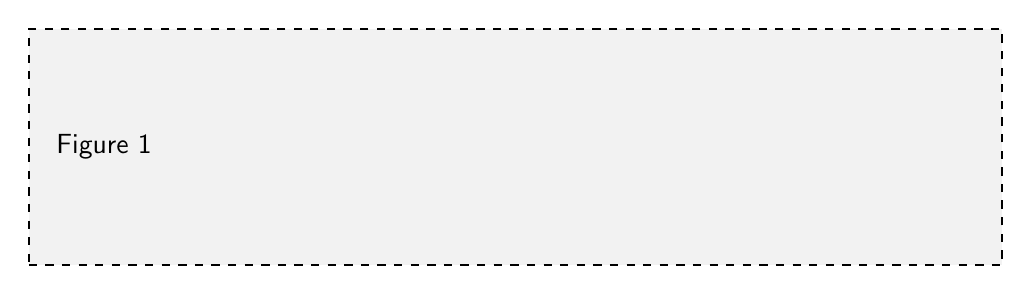
\begin{tikzpicture}
    \node[draw, fill=black!5, dashed, thick,
          text width=\textwidth, minimum height=3cm] at (0,0) {~~\sf Figure 1};
  \end{tikzpicture}
  \caption{Full width figure ({\tt width=\textbackslash headwidth}) uses a
    regular caption}
  \label{fig:1}
\end{figure}

\begin{figure}[htbp]
  \marginnote{
    \caption{Side caption can be easily inserted using the {\tt \textbackslash
        marginnote} command. Note that you may have to slightly adjust the
      vertical offset to align caption and the top of figure which is the
      recommended layout.}}[-2.5em]
  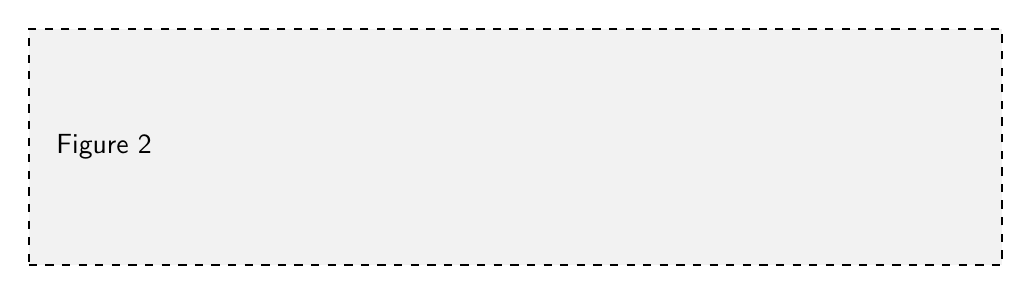
\begin{tikzpicture}
    \node[draw, fill=black!5, dashed, thick,
          text width=\textwidth, minimum height=3cm] at (0,0) {~~\sf Figure 2};
  \end{tikzpicture}
  \label{fig:2}
\end{figure}

\begin{figure}[htbp]
  
\begin{tikzpicture}
    \node[draw, fill=black!5, dashed, thick,
          text width=.99\headwidth, minimum height=3cm] at (0,0) {~~\sf Figure 3};
  \end{tikzpicture}
  \marginnote{
    \caption{Full width figure using a side caption}}[-2.0em]
  \label{fig:3}
\end{figure}

\section{Commands}

The template defines various commands to help with the writing.
\begin{lstlisting}
\citep{Rougier:2017}\sidecite{Rougier:2017}
\end{lstlisting}

\lipsum[3]


\addcontentsline{toc}{section}{References}
\renewcommand*{\bibfont}{\footnotesize \sffamily}
\printbibliography

\end{document}
